\chapter{Evaluation}
\label{cha:evaluation}
In this chapter we present the evaluation of the work done. This will measure the performance and scalability of the integration by presenting benchmarks of the running system.\par
	Section \ref{sec:operation_propagation_time} measures how the number of operations each message contains influences the time needed to propagate them. Section \ref{sec:meta-data_size} shows how the meta-data stored in Antidote increase with the operations executed in the system.

\section{Operation Propagation Time}
\label{sec:operation_propagation_time}
In this section we will focus on measuring the propagation time of operations between Legion and Antidote and how it fluctuates with other variables. In this test scenario, we use one Antidote instance, one Legion object server instance, one Antidote client and one Legion node. All the system components are located in the same local network. To run these tests we used two machines, both with a cpu of four cores, one running at 2.4GHz with 8GB of ram and the other running at 3.9GHz with 16GB of ram. The experiment consists in having our client saving the current time in one set. The update is sent and when the other client detects to have received the update, saves the time and makes the difference between the two times. This measures the latency of operation propagation.\par
	First, Figure \ref{graph1} measures the operation propagation time scaling with the number of operations in each message. As we can see, the time it takes to propagate a message, increases with the number of operations that each message contains. When propagating messages from Legion to Antidote, the time required increases nearly linearly with the number of operations. On the other hand, when propagating messages from Antidote to legion, the time required does not grow as fast, only increasing slightly with the number of operations in each message.\par
	The reason for this is that when propagating operations from Legion to Antidote, it is necessary to record more data that is create in Legion into Antidote, while in the other direction the data was already in Antidote.

\begin{figure}[H]
\centering
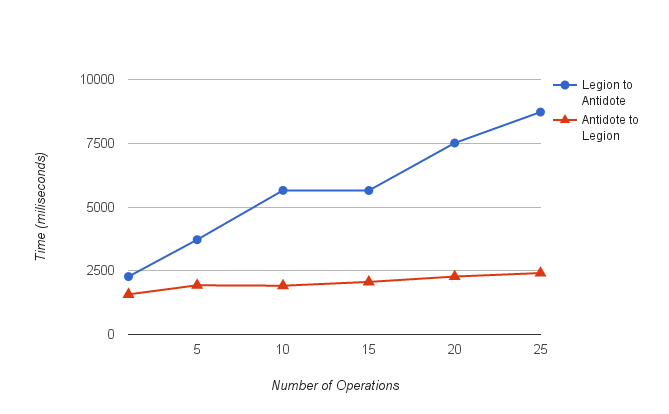
\includegraphics[scale=0.7]{files/graph1.png}
\caption{Propagation time scaling with operations per message}
\label{graph1}
\end{figure}

\begin{figure}[H]
\centering
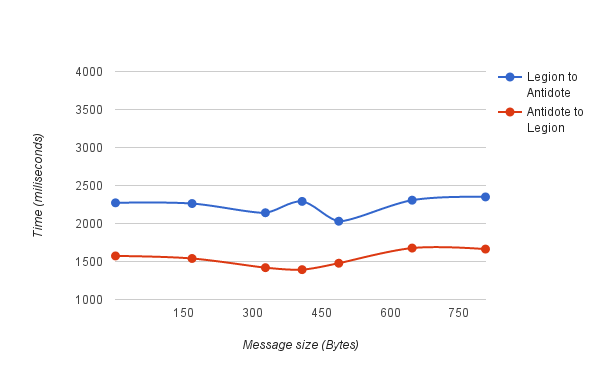
\includegraphics[scale=0.7]{files/chart2.png}
\caption{Propagation time scaling with message size}
\label{chart2}
\end{figure}

Second, Figure \ref{chart2} evaluates the scalability of the message propagation time with the size of the message. In this test scenario, we calculate the size of the messages based on the number of elements added to a set and the size of each element. As we can see, the time needed to propagate a message is constant with the growth of the message size. Although the message size does not affect the propagation time in either direction, Legion to Antidote synchronization requires more time compared to the Antidote to Legion message propagation. The reason for message size having little impact resides in the fact that the overhead in processing is per operation, i.e., for each operation a number of additional steps need to be executed independently of the operation size.\par
	In the next evaluation scenario, we will measure the scalability of propagating data between two separate Legion groups that can only share information via Antidote. In order to do so, the first evaluation setup is composed by one Antidote instance, two Legion object server instances and two Legion nodes connected to separate object servers. The second setup uses two Antidote nodes connected to different Legion groups. In this scenario, the time measured starts when a Legion node issues an update and ends when the other group's Legion node receives the update. In order to propagate updates between Legion groups, Antidote is used as a synchronization point, where one Legion node updates the storage system, and the other fetches the updates. In Figure \ref{chart4} we measure the time of propagating messages between the two Legion nodes with an increasing number of operations in each message. As we can see, the time needed scales nearly linearly with the number of operations, having a consistent result with the results presented before.\par
	Finally, Figure \ref{chart5} we present the scalability of the message propagation time with the size of each message. Similarly to Figure \ref{chart2}, the growth of the message size does not affect the propagation time between the two Legion nodes.

\begin{figure}[H]
\centering
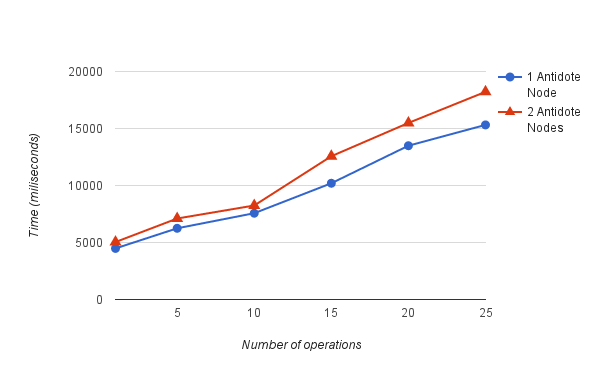
\includegraphics[scale=0.7]{files/chart4.png}
\caption{Propagation time scaling with operations per message between two Legion groups}
\label{chart4}
\end{figure}

\begin{figure}[H]
\centering
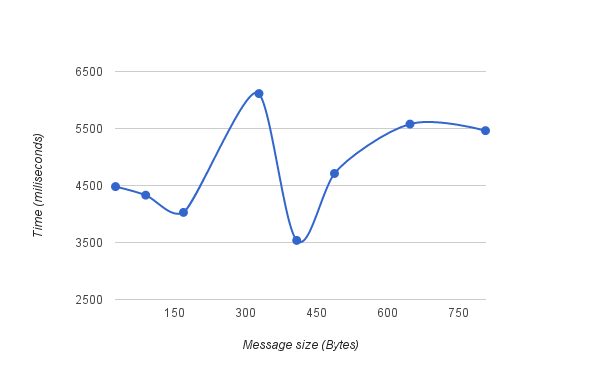
\includegraphics[scale=0.7]{files/chart5.png}
\caption{Propagation time scaling with message size between two Legion groups}
\label{chart5}
\end{figure}

\section{Meta-Data Size}
\label{sec:meta-data_size}
As explained in section \ref{sec:integration_challenges}, in order to keep a correspondence between Legion and Antidote identifiers, there is a need to store meta-data information in the Antidote nodes. In this section we measure the size of this meta-data along with its scalability as the system runs. Figure \ref{chart3} shows the size of meta-data stored in an Antidote node. In this test scenario, we consider write and delete operations, as these separately will influence the final size of meta-data. The blue line represents a workload where 50\% of the updates are writes and the other 50\% are deletes. On the other hand, the red line has a more write intensive workload, with 80\% writes and 20\% deletes.\par
	As expected, the meta-data size stored increases with the number of operations. In the red workload, the growing is continuously linear. The blue workload also grows continuously, but needs less memory. This is due to the unique tokens that are erased when a delete operation is issued, making the only stored data the operation identifiers.\par
	The always growing tendency of the meta-data derives from the operation identifiers that will keep stacking as the system runs. This calls for the need of including a garbage collector to clean the metadata that is no longer needed from time to time.

\begin{figure}[H]
\centering
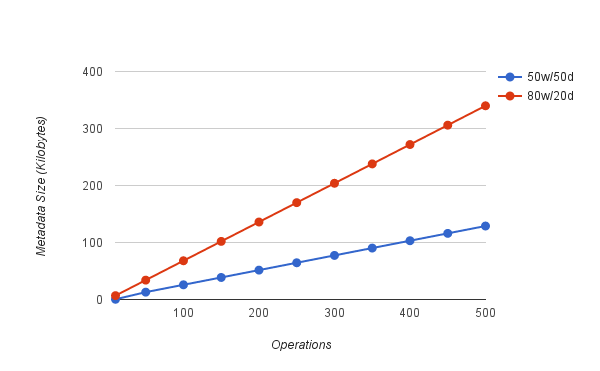
\includegraphics[scale=0.7]{files/chart3.png}
\caption{Meta-data size scaling with propagated operations}
\label{chart3}
\end{figure}

